\section{Introduction}

Traditional HPC compute clusters are created by combining separate compute servers over network fabric devices to form the cluster.  Each individual compute server is provisioned with its own CPUs, memory devices, accelerator cards, and storage devices to incorporate as many different application runtime requirements as possible.<cite >. This need to incorporate 'all of the options' makes traditional HPC architectures less flexible, inefficient, and can lead to situations where application jobs more prone to run-time failure.    
For example, design considerations that lead to an under-estimation of compute server memory resources can cause out-of-memory conditions.  In another example, IO server memory oversubscription can result in filesystem failure can occur due to virtual memory page swap thrashing and eventually application failure when the dynamic addition of memory would be able to help mitigate this problem.  

Yet another issue with current HPC architecture that is a result of architectural inflexibility frequently results in overprovisioned or stranded resources.  Stranded resources are defined as resources that are either on a compute server that is unavailable to a workload, or that have been assigned to a workload that isn't making use of them.  These resources have been made to be unavailable to be used by other workloads. Overprovisioned resources are those that are either underused, or unused and idle for the current workloads but still draw energy and cooling.  Energy wasted in data centers is becoming an increasingly important issue.  {cite https://www.energy.gov/eere/buildings/data-centers-and-servers } 
The facility costs scale of large HPC systems, cooling and energy usage become  
  (4% of energy produced are used in data centers, 2% of energy usage was used in data centers, 2 years ago <>
  <https://www.dw.com/en/data-centers-energy-consumption-steady-despite-big-growth-because-of-increasing-efficiency/a-60444548>
  <https://www.marketscreener.com/quote/stock/VMWARE-INC-58476/news/VMware-Why-Energy-Sobriety-Should-Be-Top-of-Mind-for-Every-Business-Leader-This-Year-42823597/>

A solution to addressing the ovprovisioning and computational efficiency limitations, as well as hardware and operating costs, of integrated, siloed, systems is the use of Composable Disaggregated Infrastructures. (Figure \ref{fig:stranded}) 

\begin{figure}
\centerline{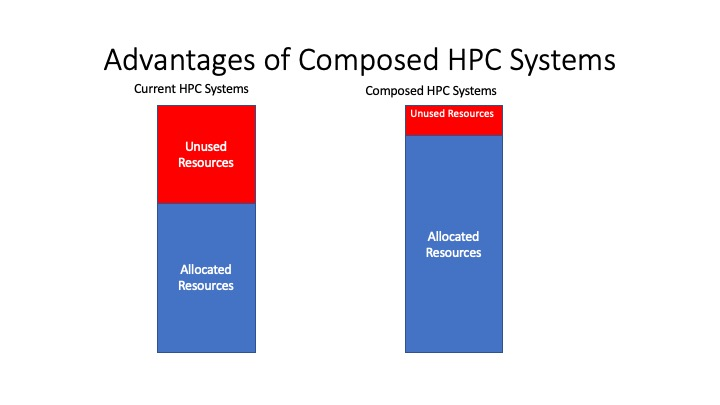
\includegraphics[width=\columnwidth]{Slide3.jpeg}}
\caption{More Efficiency in Composable HPC Use of Resources.} 
\label{fig:stranded}
\end{figure}

Disaggregate computational resources are not statically provisioned in servers, but instead are physically disaggregated and connected through High-speed/low-latency network fabrics.  These resources can be dynamically provisioned and reprovisioned to client applications, as needed and are thus not only more efficient to manage by removing unnecessary hardware, but help reduce energy consumption and datacenter cooling costs.  In this type of architecture, shared 'pools' are created that are accessed across high-speed, low latency fabrics. Figure \ref{fig:Pools}


\begin{figure}
\centerline{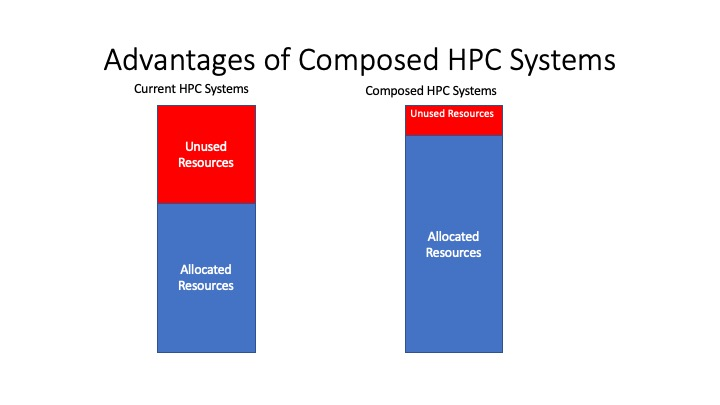
\includegraphics[width=\columnwidth]{Slide3.jpeg}}
\caption{More Efficiency in Composable HPC Use of Resources.} 
\label{fig:stranded}
\end{figure}

\begin{figure}
\centerline{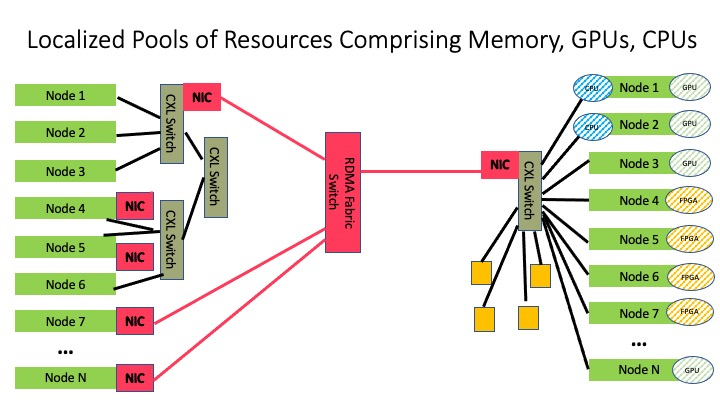
\includegraphics[width=\columnwidth]{Slide4.jpeg}}
\caption{Localized Disaggregated Resource Pools Connected by Fabrics.} 
\label{fig:Pools}
\end{figure}

Network disaggregation is already common for storage devices (e.g., NVMe-oF); current trends are pushing this paradigm further, extending it to computational engines, memory elements, accelerators… eventually to all forms of compute resources required by modern HPC applications.  

However, disaggregated resource types are increasingly being accessed over an increasing number of fabric types and technologies; and being able to fully manage these resources in a dynamic, heterogenous environment requires managing those fabrics and the hardware resources that may be accessed thereon. The management and optimization of such a diverse set of fabrics and fabric technologies to realize the benefits of Composable Disaggregated Infrastructures is quickly becoming a complex issue to solve for infrastructure managers, especially in heterogenous multi-vendor environments, with multiple vendor-sourced hardware and the ever-expanding collection of proprietary APIs and tools. Currently, there is no common open-source manager interface or model available to configure the resource pools and the fabrics that link them with applications that need them. So every tool & every middleware library provider needs unique calls to specific fabric managements stack for each available fabric You end up with very diverse administration domains w/ administrators having to manage each fabric differently through different tools.

The industry needs interoperatbility through common interfaces to enavle managers to efficiently connect workloads iwsth resources in a dynam3eic ecosystem withoyut having to worrry about the underlying network interconnect.  This paper describes an Open Fabric Management framework, an API, tool set, and central repository designed for managing comnposable resources over multiple fabrics for manipulating resources using client-friendly abstractions, and configuring fabric interconectsso that workloads can be linked with disaggregated resources over dynamic fabric infrastructrues.

  
 

\begin{table*}
  \caption{An overview of several performance profiles, example leading representative benchmarks, and degree of performance isolation typically expected between nodes and/or tasks by HPC users.}
  \label{Table:profiles}
  \begin{center}
%\begin{tabular}{|p{0.22\linewidth}|p{0.45\linewidth}|p{0.18\linewidth}|p{0.15\linewidth}|}
\begin{tabular}{|l|l|l|l|}
\hline
{\bf Profile} & {\bf Description} & {\bf Benchmark} & {\bf Isolation} \\
\hline
CPU-bound & Heavy use of CPU and accelerators & HPL~\cite{hpl} & Strong\\
\hline
Memory-bound & Reads and writes to main memory & \raggedright STREAM~\cite{stream}, HPCG~\cite{hpcg} & Strong\\
\hline
Network-bound & Sending and receiving data among nodes in a task & \raggedright Intel MPI Benchmarks~\cite{imb} & Medium-to-Strong\\
\hline
IOPs-bound & Many small reads/writes to a few files & IOR-hard~\cite{io500} & Weak\\
\hline
Bandwidth-bound & Large reads/writes to a few files & IOR-easy~\cite{io500} & Weak\\
\hline
Metadata-bound & Many small reads/writes to may files & mdtest~\cite{ior} & Weak \\
\hline
\end{tabular}
\end{center}
\end{table*}


